\section{Detailed Dataset Construction, Generation, and Quality Checks}
\label{app:data}

\paragraph{A.1 Source corpora, sampling, and release scope.}

\begin{table}[h]
  \centering
  \small
  \begin{tabular}{@{}p{2.0cm}p{1.1cm}p{0.9cm}p{2.2cm}@{}}
    \toprule
    \textbf{Corpus} & \textbf{Lang.} & \textbf{Inst.} & \textbf{Resource use} \\
    \midrule
    iSarcasmEval (SemEval-2022 T6) & English & 3{,}467 & SarcTrain; GenTrain; DualTest$^{\ast}$ \\
    CSC & English & 6{,}878 & SarcTrain; GenTrain \\
    ToSarcasm & Chinese & 3{,}898 & SarcTrain; GenTrain; DualTest$^{\ast}$ \\
    News Headlines v2 & English & 28{,}619 & SarcTrain \\
    Open Chinese Internet Sarcasm Corpus & Chinese & 2{,}000 & SarcTrain \\
    \bottomrule
  \end{tabular}
  \caption{Input corpora and resource use. The instance counts refer to the 44{,}862-record pooled collection; $^{\ast}$DualTest uses separate official test splits excluded from these counts. Genres and annotations are iSarcasmEval (tweets, speaker self-annotation), CSC (conversational responses), ToSarcasm (topic comments, third-party annotation), News Headlines (distant supervision from The Onion / HuffPost), and the Open Chinese Corpus (Weibo, third-party annotation).}
  \label{tab:sources}
\end{table}

\Tabref{tab:sources} lists the input corpora and how each is used. The pooled collection contains 44{,}862 instances in total (86.9\% English and 13.1\% Chinese). SarcTrain is balanced across the four language $\times$ sarcasm strata by downsampling the two English strata and the Chinese non-sarcastic stratum, then sampling 104 additional Chinese sarcastic records with replacement. The Chinese sarcastic source pool contains 2{,}396 records corresponding to 2{,}394 distinct stored text values; after expansion to 2{,}500 records, its text-duplication rate is 4.24\% (A.3).

The iSarcasmEval and CSC repositories display MIT licenses and the News Headlines v2 Kaggle release states CC BY 4.0, whereas we did not identify explicit redistribution licenses in the releases we accessed for ToSarcasm or the Open Chinese Internet Sarcasm Corpus. We therefore do not redistribute human-authored text from the latter two sources. Accordingly, we treat only eligible AI-generated text, labels and metadata, and reconstruction scripts that require users to obtain the human-authored corpora from their original sources as redistributable project artifacts.

\paragraph{A.2 Language $\times$ source $\times$ sarcasm distribution of DualTest.} The retained counts are reported in \Tabref{tab:dualtest-dist}.

\begin{table}[H]
  \centering
  \small
  \begin{tabular}{@{}llcc@{}}
    \toprule
    \textbf{Lang.} & \textbf{Source} & \textbf{Sarc.} & \textbf{Non-sarc.} \\
    \midrule
    English & Human & 200 & 1{,}200 \\
    English & AI & 192 & 1{,}174 \\
    Chinese & Human & 623 & 349 \\
    Chinese & AI & 587 & 339 \\
    \bottomrule
  \end{tabular}
  \caption{Language $\times$ source $\times$ sarcasm distribution of DualTest. Human-authored texts use dataset sarcasm annotations; AI-generated texts use prompt-specified style labels.}
  \label{tab:dualtest-dist}
\end{table}

\paragraph{A.3 Data quality checks.} Automated checks confirm language and sarcasm-label balance across the five SarcTrain folds. AuthTrain contains 9{,}996 complete human--AI pairs and three unmatched human instances. Record-level matching finds that neither SarcTrain nor AuthTrain shares records with either the human or AI side of DualTest.

SarcTrain's text-duplication rate is 0.34\% for English and 2.16\% for Chinese. Chinese duplication is concentrated in the sarcastic stratum (4.24\%; non-sarcastic stratum: 0.08\%) and results primarily from the oversampling used to fill that stratum (A.1). Because oversampling precedes fold assignment, for 86 of the 104 added records, another copy originating from the same source record is assigned to a different fold. The two counting rules are summarized in \Tabref{tab:dup-rules}.

\begin{table}[H]
  \centering
  \footnotesize
  \setlength{\tabcolsep}{3pt}
  \begin{tabular}{@{}p{3.25cm}ccc@{}}
    \toprule
    \textbf{Counting rule} & \textbf{Dup. sets} & \textbf{Records} & \textbf{Cross-fold} \\
    \midrule
    Exact stored text; oversampled copies included & 116 & 241 & 98 \\
    Case/whitespace normalized; added copies excluded & 19 & 46 & 16 \\
    \bottomrule
  \end{tabular}
  \caption{Duplicate-record counts under the two counting rules used in the data-quality audit.}
  \label{tab:dup-rules}
\end{table}

The first rule underlies the reported duplication rates; the second isolates pre-existing duplicates after the added copies are removed. These relationships are relevant to fold-based checkpoint selection but do not place the affected training or validation records into DualTest.

\phantomsection\label{app:a4}\paragraph{A.4 AI generation protocol.} The AI-generated texts in AuthTrain, the primary DeepSeek-generated DualTest AI subset, and the separate Qwen3.5 transfer subset are produced by locally deployed models through the Ollama API. The model deployed under the Ollama tag \texttt{deepseek-r1:8b} generates AuthTrain and the primary DualTest AI subset. Qwen3.5-9B, deployed under the tag \texttt{qwen3.5:9b}, generates the transfer subset evaluated with the same detectors without retraining. Both models use temperature $= 0.8$, top-$p = 0.95$ \citep{holtzman2020nucleus}, and a maximum output length of 500 tokens. Generation instructions use four templates defined by language $\times$ style, with style determined by the seed instance's sarcasm label. The templates constrain output style and length to 20--80 Chinese characters or 10--50 English words. These constraints are intended to reduce, but do not eliminate, source differences in length, so \Appref{app:repr} separately repeats the representation correlation analysis within length tertiles. The complete Chinese sarcastic template used in the experiment is reproduced verbatim below:

\begin{quote}\small\ttfamily
【任务】生成一条讽刺风格的评论\\
【主题】\{seed\}\\
【要求】\\
- 直接给出简短的评论，不要解释思路或分析\\
- 风格要讽刺、幽默、夸张\\
- 表达与主题相关的观点即可，不必追求严谨\\
- 20-80字为佳\\
【评论】
\end{quote}

Its Hanyu Pinyin transliteration is:

\begin{quote}\small\ttfamily
[Renwu] Shengcheng yi tiao fengci fengge de pinglun\\
{[Zhuti]} \{seed\}\\
{[Yaoqiu]}\\
- Zhijie geichu jianduan de pinglun; buyao jieshi silu huo fenxi\\
- Fengge yao fengci, youmo, kuazhang\\
- Biaoda yu zhuti xiangguan de guandian ji ke; bubi zhuiqiu yanjin\\
- 20--80 zi wei jia\\
{[Pinglun]}
\end{quote}

Its English translation is:

\begin{quote}\small\ttfamily
[Task] Generate a sarcastic comment\\
{[Topic]} \{seed\}\\
{[Requirements]}\\
- Directly provide a short comment; do not explain your reasoning or analysis\\
- The comment should be sarcastic, humorous, and exaggerated\\
- It is sufficient to express a viewpoint related to the topic; the comment need not be rigorous\\
- Preferably 20--80 Chinese characters\\
{[Comment]}
\end{quote}

The Chinese non-sarcastic template differs only in the style line, which requests a normal, natural style. The English templates use the same field structure and request either a sarcastic, humorous, exaggerated style or a normal, natural style, with a length limit of 10--50 words.

Post-processing removes \texttt{<think>\dots</think>} segments, reasoning prefaces such as ``好的'' (\textit{hǎo de} `okay'), ``嗯'' (\textit{ń} `hmm'), ``Okay,'' ``Let me,'' and ``First,'' and Markdown markup. Outputs that still exceed the length limit or exhibit cyclic repetition after repeated generation attempts are discarded. AuthTrain retains 9{,}996 AI counterparts from 9{,}999 seeds; DualTest retains 2{,}292 counterparts from 2{,}372 seeds.

The Qwen3.5-generated AI test subset has no generation failures, yielding 1{,}550 AI $\times$ non-sarcastic instances rather than 1{,}513. Generator-specific rates therefore use the full set of retained outputs for each generator rather than an identical seed intersection. For this run, Ollama thinking mode is disabled (\texttt{think = false}) to prevent the reasoning process from exhausting the output budget. The same post-processing removes any inline chain-of-thought from the \texttt{deepseek-r1:8b} outputs.

\paragraph{A.5 SFT training and generation evaluation.} After eligibility filtering, 5{,}257 records labeled as sarcastic remain for generation-task construction (2{,}972 English; 2{,}285 Chinese). After shuffling with seed 42, we sample 40\% of these records, yielding 2{,}103 instances (1{,}214 English; 889 Chinese); language balancing then samples 325 additional Chinese records with replacement, producing GenTrain (2{,}428; 1{,}214 per language). By prompt type, it comprises 374 rewriting instances, 839 response instances, and 1{,}215 comment instances. Generation evaluation uses a separately constructed set of 300 prompts that is not part of the GenTrain training--validation split (180 Chinese and 120 English): the Chinese task is to generate a sarcastic comment on a given topic, and the English task is to rewrite a normal sentence as a sarcastic one. Language and generation task are therefore not independently varied. This set is used for detector scoring and all three LLM evaluations in \Sref{sec:eval}.

\section{Hyperparameters and Training Details}
\label{app:hyper}

\paragraph{B.1 Discriminative learning rates.}

\begin{table}[h]
  \centering
  \small
  \setlength{\tabcolsep}{1.5pt}
  \begin{tabular}{@{}>{\raggedright\arraybackslash}p{2.35cm}cccc@{}}
    \toprule
    \textbf{Configuration} & \textbf{Enc.} & \textbf{Inter.} & \textbf{Sarc.} & \textbf{MGTD} \\
    \midrule
    Plain dual-head & $5\times10^{-7}$ & --- & $5\times10^{-6}$ & $1\times10^{-5}$ \\
    Plain sarcasm-only & $5\times10^{-7}$ & --- & $5\times10^{-6}$ & --- \\
    Plain MGTD-only & $5\times10^{-7}$ & --- & --- & $1\times10^{-5}$ \\
    Interaction-projection dual-head & $5\times10^{-7}$ & $5\times10^{-6}$ & $5\times10^{-6}$ & $5\times10^{-6}$ \\
    RCNN dual-head & $5\times10^{-7}$ & $5\times10^{-6}$ & $5\times10^{-6}$ & $5\times10^{-6}$ \\
    RCNN sarcasm-only & $5\times10^{-7}$ & $5\times10^{-6}$ & $5\times10^{-6}$ & --- \\
    RCNN MGTD-only & $5\times10^{-7}$ & $5\times10^{-6}$ & --- & $1\times10^{-5}$ \\
    \bottomrule
  \end{tabular}
  \caption{Discriminative learning rates for the dual-head and task-specific controls. The plain setting is also used in the backbone comparison. A dash denotes an inactive module or task head.}
  \label{tab:lr}
\end{table}

\Tabref{tab:lr} lists the per-module learning rates. The sarcasm-head learning rate is fixed at $5\times10^{-6}$ in every configuration with an active sarcasm head. The MGTD-head rate is $1\times10^{-5}$ for the plain dual-head model and the plain and RCNN MGTD-only controls, compared with $5\times10^{-6}$ for the RCNN and interaction-projection dual-head models. Thus, the core joint-versus-sarcasm-only comparisons retain the same sarcasm-specific rates within each architecture. Because the RCNN joint-versus-MGTD-only comparison also changes the MGTD-head learning rate, it is reported descriptively rather than as an optimization-matched estimate of transfer; cross-configuration differences can likewise reflect optimization settings. Early stopping uses the normalized joint validation loss of Equation~\ref{eq:stop} for dual-head models and the task's own validation loss for the task-specific controls, with a patience of five epochs in both procedures.

\paragraph{B.2 Shared training hyperparameters.} Training uses \texttt{torch.optim.AdamW} with default PyTorch betas $(0.9,0.999)$ and $\epsilon=10^{-8}$, weight decay 0.01, and parameter-group learning rates in B.1. We implement a linear 200-step warmup followed by a constant learning rate using PyTorch's \texttt{LambdaLR}. Training runs for at most 10 epochs, with an early-stopping patience of 5 and gradient clipping at 1.0. The physical batch size is 4 with gradient accumulation over 4 steps, giving an effective batch size of 16 for the active task. The MGTD:sarcasm sampling ratio is 2:1, and the sarcasm class weights are $[1.0, 2.5]$ for the non-sarcastic and sarcastic classes, respectively. The task ratio and class weights were fixed before DualTest evaluation. The optimization settings reported here and in B.1 were selected based on prior practice and hardware constraints. We did not conduct a systematic hyperparameter search, and DualTest was not used to choose these optimization settings. The normalized joint validation loss is $0.5 \times$ [sarcasm validation loss / first-epoch value] $+ 0.5 \times$ [MGTD validation loss / first-epoch value]. The single-head controls process the full sarcasm training fold each epoch, whereas the dual-head models draw sarcasm batches under the 2:1 task-mixing schedule.

Detector inputs use a maximum sequence length of 512 tokens. In the RCNN module, a width-$k$ convolution uses padding $\lfloor k/2\rfloor$ followed by ReLU. Global max pooling covers all convolution positions; no post-convolution padding mask is applied.

All fold-based runs use a seed equal to 42 plus the fold index and share the same fold assignments and random-seed values across architectures and ablations. The same fixed AuthTrain 90/10 split is reused in all five runs; only the SarcTrain validation fold changes. For each configuration, the epoch count used to train its final model is the mode of its five best epoch counts plus one, capped at 10 epochs; the resulting counts range from 3 to 10 across configurations. This mode-plus-one refitting rule was fixed before DualTest evaluation. The final model uses all applicable training data, a seed offset of $+1000$, no validation set, and no early stopping. Tables~\ref{tab:backbone} and~\ref{tab:ablation} report five-run means and standard deviations, whereas \Tabref{tab:quadrant} and the subsequent fixed-model analyses use separately trained final models.

\paragraph{B.3 Model sizes and computational environment.} The encoders have approximately 178M (mBERT), 278M (XLM-RoBERTa-base), 184M (DeBERTa-v3-base), and 435M (DeBERTa-v3-large) parameters; the SFT generator Qwen3-8B has about 8B parameters, of which QLoRA updates only low-rank adapters. Detector training and inference are performed on a single NVIDIA GeForce RTX 3090 (24\,GB; driver 570.124.04). Across the fold-based backbone, architecture, and ablation experiments and the training of final models, detector training and inference take approximately 170 GPU-hours on this single GPU. This figure excludes local text generation through Ollama, SFT (about two hours), and the representation analyses, which run on CPU. A single detector run takes from a few minutes to a few hours. The software environment is Python 3.11.0, PyTorch 2.9.0 (CUDA 12.8; cuDNN 9.10.2), transformers 4.57.1, NumPy 2.3.5, SciPy 1.17.0, scikit-learn 1.8.0, pandas 2.3.3, peft 0.18.0, and datasets 4.4.1. AI-generated texts are produced locally through Ollama (\hyperref[app:a4]{Appendix~A.4}); LLM evaluation uses API calls made in May 2026 (\hyperref[app:c4]{Appendix~C.4}).

\paragraph{B.4 SFT (QLoRA).} We fine-tune Qwen3-8B using QLoRA \citep{dettmers2023qlora}, with 4-bit loading and bfloat16 computation. The LoRA configuration \citep{hu2022lora} uses rank 64, alpha 16, and dropout 0.0 and targets \texttt{q\_proj}, \texttt{k\_proj}, \texttt{v\_proj}, \texttt{o\_proj}, \texttt{gate\_proj}, \texttt{up\_proj}, and \texttt{down\_proj}. The maximum sequence length is 2{,}048, with gradient checkpointing enabled. Training uses a learning rate of $5\times10^{-5}$, three epochs, batch size 1, gradient accumulation 8, and a warmup ratio of 0.05. After language balancing, a seed-42 split holds out 15\% of GenTrain for validation; validation loss selects the checkpoint. Because language-balancing oversampling precedes the split, duplicated Chinese records may occur in both partitions.

\section{Complete Experimental Results}
\label{app:results}

Sections C.1--C.3 supplement the detector and subgroup analyses in \Sref{sec:exp}, while Sections C.4--C.8 provide protocols, controls, and additional results for the exploratory LLM-judge comparison in \Sref{sec:eval}.

\phantomsection\label{app:c1}\paragraph{C.1 Macro-averaged F1 (supplement to \Tabref{tab:backbone}).} Under the same five-run protocol, the RCNN macro-averaged F1 scores computed from each run's confusion matrix are \textbf{0.6678 $\pm$ 0.036} for sarcasm and \textbf{0.9298 $\pm$ 0.005} for MGTD. Sarcasm macro-F1 is higher than its positive-class F1 (0.6309) because the non-sarcastic majority class has a higher F1. These values supplement the positive-class results in \Sref{sec:backbone}; because macro-F1 is not reported for every configuration, they are not used for cross-configuration ranking.

\paragraph{C.2 Complete source $\times$ sarcasm subgroup results for the MGTD head (including MGTD-only controls).} The reporting convention matches \Tabref{tab:quadrant} (recall for human subsets; false-positive rate for AI subsets).

\begin{table}[h]
  \centering
  \small
  \setlength{\tabcolsep}{2.5pt}
  \begin{tabular}{@{}p{2.35cm}cccc@{}}
    \toprule
    \textbf{Model} & \textbf{H$\times$s} & \textbf{H$\times$n} & \textbf{AI$\times$s} & \textbf{AI$\times$n} \\
    \midrule
    Plain dual-head & 91.4 & 91.5 & 3.6 & 6.1 \\
    Interaction-projection dual-head & 85.4 & 85.4 & 1.8 & 4.1 \\
    RCNN dual-head & 94.8 & 93.2 & 5.5 & 6.6 \\
    Plain MGTD-only & 90.4 & 86.6 & 4.1 & 4.2 \\
    RCNN MGTD-only & 90.5 & 92.4 & 3.6 & 5.7 \\
    \bottomrule
  \end{tabular}
  \caption{MGTD-head results across the four source $\times$ sarcasm subgroups (\%): recall for human (H) subsets, false-positive rate for AI subsets. s = sarcastic, n = non-sarcastic.}
  \label{tab:auth-quadrant}
\end{table}

In every subgroup, each MGTD-only control differs from its corresponding dual-head model by fewer than ten percentage points. No comparably large subgroup error appears on the MGTD side, consistent with \Sref{sec:quadrant}.

When the same detectors evaluate the Qwen3.5-generated AI test subset without retraining, the MGTD head again shows no comparable subgroup increase: AI $\times$ non-sarcastic false-positive rates are 0.9\%, 1.3\%, and 0.5\% for the plain, interaction-projection, and RCNN configurations; AI $\times$ sarcastic rates are at most 0.4\%; and overall MGTD F1 scores are 0.952, 0.917, and 0.965.

\phantomsection\label{app:c3}\paragraph{C.3 Complete source $\times$ sarcasm subgroup results: confidence intervals, paired tests, language strata, and generator transfer (\Sref{sec:quadrant}--\Sref{sec:crossgen}).} For each separately trained final model, we quantify uncertainty from the test instances with Wilson 95\% intervals for subgroup rates and 95\% percentile intervals from 10{,}000 instance-level bootstrap samples for F1. The instance-level bootstrap resamples text instances independently and does not preserve human--AI seed pairs. These intervals do not include uncertainty from training, generator sampling, corpus construction, or human--AI pairing. They complement the between-run standard deviations in \Tabref{tab:ablation} and \Tabref{tab:backbone}. All values use the final model for each architecture and follow the reporting convention of \Tabref{tab:quadrant}. Across the five final models, sarcasm AUC within AI-generated texts ranges from 0.82 to 0.88.

\begin{figure*}[t]
  \centering
  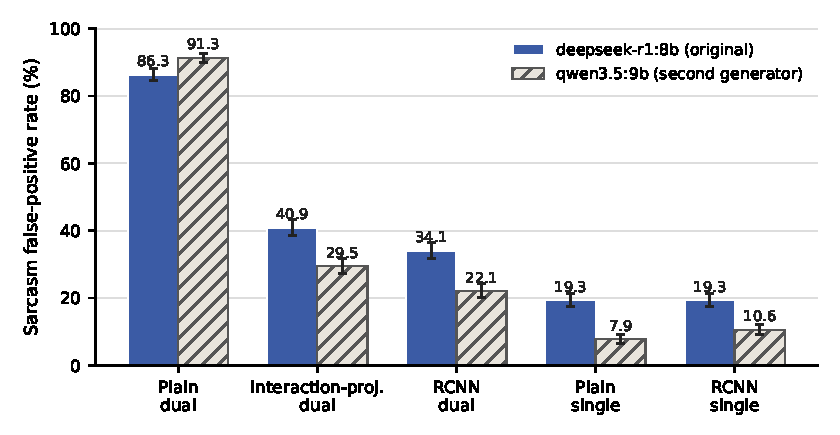
\includegraphics[width=\textwidth]{figures/fig1_quadrant_failure.pdf}
  \caption{Sarcasm false-positive rates on AI-generated texts prompted to be non-sarcastic, for five detectors and two generators. Error bars are Wilson 95\% intervals conditional on each fixed model.}
  \label{fig:quadrant}
\end{figure*}

\Figref{fig:quadrant} plots these subgroup rates for both generators, and \Tabref{tab:wilson} gives the corresponding intervals. For both matched model pairs, the false-positive rate remains higher under the joint procedure on the Qwen3.5-generated texts, although the magnitudes differ.

\begin{table}[h]
  \centering
  \footnotesize
  \setlength{\tabcolsep}{1.5pt}
  \begin{tabular}{@{}>{\raggedright\arraybackslash}p{2.25cm}cc@{}}
    \toprule
    \textbf{Model} & \textbf{DeepSeek} & \textbf{Qwen3.5} \\
    \midrule
    Plain dual-head & 86.3 [84.5, 88.0] & 91.3 [89.8, 92.6] \\
    Interaction-projection dual-head & 40.9 [38.5, 43.4] & 29.5 [27.3, 31.8] \\
    RCNN dual-head & 34.1 [31.8, 36.5] & 22.1 [20.1, 24.3] \\
    Plain single-head & 19.3 [17.4, 21.4] & 7.9 [6.6, 9.3] \\
    RCNN single-head & 19.3 [17.4, 21.4] & 10.6 [9.2, 12.3] \\
    \bottomrule
  \end{tabular}
  \caption{Wilson 95\% intervals for the sarcasm false-positive rate on AI-generated texts prompted to be non-sarcastic (two generators; \%).}
  \label{tab:wilson}
\end{table}

Paired McNemar tests use predictions on the same DeepSeek-generated AI $\times$ non-sarcastic texts. The discordant-pair counts are 1{,}021 / 7 for plain dual vs.\ plain single, 239 / 15 for RCNN dual vs.\ RCNN single, 805 / 15 for plain dual vs.\ RCNN dual, and 203 / 100 for the interaction-projection dual-head model vs.\ the RCNN dual-head model (all $p < .001$). The discordant counts and absolute rate differences provide the substantive effect-size information.

\begin{table*}[t]
  \centering
  \small
  \setlength{\tabcolsep}{6pt}
  \begin{tabular}{@{}llrccc@{}}
    \toprule
    \textbf{Model} & \textbf{Lang.} & \textbf{$n$} & \textbf{Dual FP; rate [CI]} & \textbf{Single FP; rate [CI]} & \textbf{$\Delta$ pp} \\
    \midrule
    Plain & en & 1{,}174 & 987; 84.1 [81.9, 86.1] & 242; 20.6 [18.4, 23.0] & $+63.5$ \\
    Plain & zh & 339 & 319; 94.1 [91.1, 96.1] & 50; 14.7 [11.4, 18.9] & $+79.4$ \\
    RCNN & en & 1{,}174 & 445; 37.9 [35.2, 40.7] & 247; 21.0 [18.8, 23.5] & $+16.9$ \\
    RCNN & zh & 339 & 71; 20.9 [17.0, 25.6] & 45; 13.3 [10.1, 17.3] & $+7.7$ \\
    \bottomrule
  \end{tabular}
  \caption{Language-stratified sarcasm false-positive rates on AI-generated texts prompted to be non-sarcastic (\%; Wilson 95\% intervals). Dual FP and Single FP give the number of false positives under the dual- and single-head models; $\Delta$ is the dual rate minus the single rate. Exact paired McNemar tests give $p<.001$ for both plain comparisons and RCNN English, and $p=2.4\times10^{-5}$ for RCNN Chinese.}
  \label{tab:lang-quadrant}
\end{table*}

\Tabref{tab:lang-quadrant} gives the language-stratified subgroup rates and \Tabref{tab:lang-f1} the corresponding per-language F1 scores. In both architectures and both language strata, the false-positive rate is higher under the joint procedure than under its matched sarcasm-only control. Language remains coupled with corpus, genre, and annotation setting, so the stratified results do not isolate a language effect.

\begin{table*}[t]
  \centering
  \small
  \setlength{\tabcolsep}{4pt}
  \begin{tabular}{@{}lcccccc@{}}
    \toprule
    \textbf{Model} & \textbf{Full set} & \textbf{Chinese} & \textbf{English} & \textbf{Human subset} & \textbf{Human$\times$zh} & \textbf{Human$\times$en} \\
    \midrule
    Plain dual-head & 0.556 & 0.746 & 0.312 & 0.586 & 0.710 & 0.374 \\
    IP dual-head & 0.643 & 0.781 & 0.420 & 0.593 & 0.739 & 0.366 \\
    RCNN dual-head & 0.663 & 0.819 & 0.429 & 0.629 & 0.774 & 0.399 \\
    Plain single-head & 0.661 & 0.750 & 0.514 & 0.612 & 0.719 & 0.434 \\
    RCNN single-head & 0.664 & 0.758 & 0.511 & 0.603 & 0.709 & 0.434 \\
    \bottomrule
  \end{tabular}
  \caption{Per-language and human-subset sarcasm F1 (final models). IP denotes the interaction-projection configuration. Bootstrap 95\% intervals for the RCNN dual-head row are given in the text below.}
  \label{tab:lang-f1}
\end{table*}

Bootstrap 95\% intervals for the RCNN dual-head sarcasm F1 scores in \Tabref{tab:lang-f1} are [.646, .680] on the full set, [.802, .836] in Chinese, [.399, .458] in English, [.605, .653] on the human subset, [.748, .798] on Human$\times$zh, and [.355, .440] on Human$\times$en.

The final RCNN dual-head model's MGTD F1 is 0.938 [0.931, 0.945] on the full set, 0.961 [0.952, 0.969] in Chinese, and 0.923 [0.912, 0.933] in English. Because the human-only subset contains no AI-authored examples, an MGTD F1 score on that subset would not measure source discrimination; \Tabref{tab:auth-quadrant} therefore reports human recall directly.

Chinese sarcasm F1 is higher than English sarcasm F1 for the RCNN model (0.819 vs.\ 0.429). This contrast also reflects differences in prevalence, genre, and annotation procedure: sarcasm prevalence is 63.8\% in Chinese but 14.2\% in English, and the English human side is dominated by author-labeled intended-sarcasm tweets from iSarcasmEval whereas the Chinese side uses topic-comment-style ToSarcasm. The positive-class F1 values should therefore not be interpreted as an isolated language effect.

The separately retrained final RCNN model's overall sarcasm F1 is 0.663, compared with 0.629 on human-authored texts alone, because the overall score also includes AI-generated texts. This point estimate differs from the five-run mean in \Tabref{tab:backbone}, which aggregates fold-based runs. Within the human subset, absolute joint-versus-sarcasm-only differences in sarcasm F1 are below 0.03 and vary in direction. The negative-transfer effect is therefore concentrated in the subgroups containing AI-generated texts, consistent with \Sref{sec:quadrant}.

False-positive rates use a threshold of 0.5. For the plain dual-head model on AI $\times$ non-sarcastic text, the median sarcasm probability is 0.767 with an interquartile range of 0.635--0.839. The distribution therefore lies mostly above the threshold rather than placing only a few cases near it. Single-head medians are 0.204 for the plain model and 0.069 for RCNN.

The coexistence of an upward score shift and substantial within-AI discrimination motivates the representation analyses in \Appref{app:repr}.

\phantomsection\label{app:c4}\paragraph{C.4 Evaluation protocol, inter-judge rank correlations, and condition-level tests (\Sref{sec:eval}).} Each sample is evaluated separately by each of the three judge APIs in one API call using the same prompt structure for all model conditions (May 2026; temperature $= 0.3$; GPT-5-nano uses its default decoding because it does not support this parameter). The prompt contains only the input and evaluated text, not the ground-truth source label. It asks for source inference followed by 1--5 ratings of sarcasm and human-likeness. The ratings are therefore obtained without ground-truth source labels, although the judges are explicitly asked to infer source before assigning the two ratings. Base and SFT outputs are evaluated separately. The judges were accessed through the model identifiers \texttt{deepseek-chat}, \texttt{gemini-2.5-flash-lite}, and \texttt{gpt-5-nano}. At the time of our May 2026 API calls, DeepSeek's April 24, 2026 API announcement identified \texttt{deepseek-chat} as routing to the non-thinking mode of DeepSeek-V4-Flash; the legacy identifier was subsequently retired on July 24, 2026 \citep{deepseek2026v4flash}.

Pairwise inter-judge rank correlations are low to moderate, with Spearman $\rho$ ranging from 0.20 to 0.38 for sarcasm (all $p < 10^{-6}$) and from 0.03 to 0.23 for human-likeness (one pair is not significant). \Tabref{tab:group-tests} reports the corresponding condition-level tests. We therefore do not treat individual-text rankings as a common gold standard. The condition-level observation rests separately on the consistent rating direction across all six setting--judge comparisons.

Outputs from the SFT model receive lower mean sarcasm ratings in all six setting--judge comparisons, and Wilcoxon signed-rank tests with Benjamini--Hochberg FDR correction \citep{benjamini1995fdr} show that five differences remain significant. The pooled correlations in \Tabref{tab:correlation} use the three-judge mean as a descriptive aggregate, while the limited pairwise rank correlations make judge-specific results necessary. Four instances each have one unparsable rating but retain two valid judge ratings, so averaging the available ratings preserves all 600 outputs in the aggregate.

\begin{table}[h]
  \centering
  \small
  \begin{tabular}{@{}lcccc@{}}
    \toprule
    \textbf{Subset} & \textbf{$n$} & \textbf{Sarc.\ $\rho$} & \textbf{Human-like $\rho$} \\
    \midrule
    Overall & 600 & $+$0.136$^{*}$ & \textbf{$-$0.212}$^{*}$ \\
    Chinese & 360 & \textbf{$-$0.020} & $-$0.218$^{*}$ \\
    English & 240 & $+$0.338$^{*}$ & $-$0.270$^{*}$ \\
    \bottomrule
  \end{tabular}
  \caption{Spearman correlations between detector probabilities and LLM-judge ratings (RCNN detector, $n = 600$ pooled over base and SFT): Sarc.\ $\rho$ compares $P(\text{sarcastic})$ with sarcasm ratings, and Human-like $\rho$ compares $P(\text{human})$ with human-likeness ratings. $^{*}$ significant; the other entries are not significant.}
  \label{tab:correlation}
\end{table}

\begin{table}[h]
  \centering
  \footnotesize
  \setlength{\tabcolsep}{3pt}
  \begin{tabular}{@{}llcccc@{}}
    \toprule
    \textbf{Judge} & \textbf{Lang.} & \textbf{$n$} & \textbf{Base} & \textbf{SFT} & \textbf{adj.\ $p$} \\
    \midrule
    DeepSeek-V4-F & en & 120 & 4.025 & 3.292 & $<$.0001 \\
    DeepSeek-V4-F & zh & 180 & 4.044 & 3.878 & .0008 \\
    Gemini-2.5-FL & en & 120 & 3.992 & 3.750 & .0008 \\
    Gemini-2.5-FL & zh & 180 & 4.028 & 3.994 & .2008$^{\ast}$ \\
    GPT-5-nano & en & 119 & 4.084 & 3.681 & $<$.0001 \\
    GPT-5-nano & zh & 180 & 3.911 & 3.517 & $<$.0001 \\
    \bottomrule
  \end{tabular}
  \caption{Condition-level tests for sarcasm ratings obtained without ground-truth source labels (Wilcoxon $+$ BH-FDR). $^{\ast}$ not significant. Averaging the three Chinese judge means gives 3.99 for base and 3.80 for SFT, as reported in \Sref{sec:eval}. GPT-5-nano lacks one English base rating (C.4: $n=119$) and three Chinese reference ratings (affecting C.5, not the C.4 Chinese row); tests use pairwise deletion.}
  \label{tab:group-tests}
\end{table}

\paragraph{C.5 Paired tests between SFT outputs and human-authored reference texts (supplementary).} These tests are performed on the Chinese subset of the 300-prompt generation evaluation ($n = 180$; three GPT-5-nano ratings are missing, leaving 177). The comparisons provide judge- and dimension-specific comparison context: for DeepSeek-V4-Flash, SFT outputs receive significantly lower human-likeness ratings than the reference texts ($-0.161$, $p = 0.0025$), whereas for GPT-5-nano, SFT outputs receive significantly higher sarcasm ratings than the reference texts ($+0.186$, $p = 0.0114$). The remaining four comparisons do not reach significance at the reported threshold. Thus, the observed reference differences vary across judges and dimensions; these tests do not estimate a judge-by-dimension interaction.

\paragraph{C.6 Plain-detector control.} With the plain detector, the Chinese sarcasm probability changes from 0.765 to 0.763 ($-0.001$), the English sarcasm probability changes from 0.843 to 0.659 ($-0.184$), and predicted human-authorship probability rises by $+0.760$ in Chinese and $+0.705$ in English. The two detectors agree on the rise in predicted human-authorship probability. The Chinese sarcasm-probability change is detector-sensitive, whereas both detectors show a decrease in English.

Overall correlations between detector probabilities and corresponding ratings are $+0.142$ for sarcasm and $-0.214$ for human-likeness. The corresponding values are $-0.037$ (not significant) and $-0.209$ in Chinese, and $+0.342$ and $-0.283$ in English. Each differs from the RCNN-detector value by at most 0.02. Negative associations between predicted human-authorship probabilities and human-likeness ratings are similar across the two detectors, whereas the condition-level sarcasm-probability change differs between the plain and RCNN detectors, especially in Chinese.

\phantomsection\label{app:c7}\paragraph{C.7 Within-condition correlations (RCNN detector).} For predicted human-authorship probability and human-likeness ratings, the base condition has $\rho = +0.03$ ($n = 300$, not significant; Chinese $+0.10$, English $-0.09$). The SFT condition has $\rho = -0.12$ ($p = 0.039$; Chinese $-0.19$, $p = 0.009$; English $-0.12$, not significant). The pooled value of $-0.212$ is driven mainly by the opposing condition-level changes: SFT raises predicted human-authorship probability by about 0.67 while lowering the mean rating. The pooled negative correlation should therefore not be interpreted as a strong instance-level inverse relationship. Within either condition, predicted human-authorship probability is not significantly positively correlated with rated human-likeness.

For sarcasm, within-condition correlations are $+0.05$ for Chinese base (not significant), $+0.15$ for Chinese SFT ($p = 0.048$), $+0.41$ for English base, and $+0.37$ for English SFT (both English values significant). Chinese alignment is therefore at most weakly positive, consistent with its near-zero pooled result.

\phantomsection\label{app:c8}\paragraph{C.8 Detector probabilities before and after SFT across the two task--language settings.} The RCNN detector assigns the following mean probabilities to base and SFT outputs:

\begin{table}[h]
  \centering
  \footnotesize
  \setlength{\tabcolsep}{2pt}
  \begin{tabular}{@{}llcc@{}}
    \toprule
    \textbf{Lang.} & \textbf{Cond.} & \textbf{$P(\text{sarcastic})$} & \textbf{$P(\text{human})$} \\
    \midrule
    Chinese & Base $\to$ SFT & 0.780 $\to$ 0.895 & 0.289 $\to$ 0.969 \\
    English & Base $\to$ SFT & 0.854 $\to$ 0.730 & 0.198 $\to$ 0.864 \\
    \bottomrule
  \end{tabular}
  \caption{Mean detector probabilities before and after SFT (RCNN detector).}
  \label{tab:sft-scores}
\end{table}

\Tabref{tab:sft-scores} reports these means. Sarcasm probabilities move in opposite directions in the Chinese comment-generation and English rewriting settings ($+0.115$ and $-0.124$, respectively), while predicted human-authorship probabilities rise sharply in both. GenTrain itself is balanced at 1{,}214 instances per language, but the evaluation settings differ in task, prompt format, source data, and sample size, all of which may contribute to the contrast.

The mean LLM-judge ratings for the human-authored reference texts are 3.77 for sarcasm and 4.17 for human-likeness; the corresponding values are 4.01 and 4.24 for the base model and 3.71 and 4.08 for SFT. From the base model to SFT, the mean human-likeness rating decreases even as predicted human-authorship probability increases, as analyzed in \Sref{sec:eval}.

\section{Illustrative Cases of Disagreement between Detector Probabilities and LLM-Judge Ratings}
\label{app:cases}

Illustrative cases were manually selected after inspecting the paired table of RCNN-detector probabilities and ratings from the three LLM judges to show large disagreements; no formal ranking or top-$k$ selection was performed. The selection is non-systematic, and the cases should not be used to estimate the prevalence of any disagreement type. Detector probabilities range from 0 to 1, and LLM-judge ratings are averaged across the three evaluators on a 1--5 scale. Long texts are shortened for display, while Chinese examples retain the original model input and provide Hanyu Pinyin transliterations and English translations in brackets.

The three disagreement types (\Tabref{tab:cases-auth}, \Tabref{tab:cases-fp}, and \Tabref{tab:cases-fn}) show, respectively, high predicted human-authorship probabilities with low LLM-judge ratings of human-likeness, high predicted sarcasm probabilities with low LLM-judge ratings of sarcasm, and the reverse sarcasm disagreement. In the first human-likeness case, AI-generated text with an obvious reasoning-style preface is nevertheless assigned predicted human-authorship probability 1.00 by the MGTD head, corresponding to the disagreement discussed in \Sref{sec:eval}.

\begin{table}[!t]
  \centering
  \footnotesize
  \setlength{\tabcolsep}{1.2pt}
  \begin{tabular}{@{}>{\centering\arraybackslash}p{1.05cm}>{\centering\arraybackslash}p{0.9cm}>{\centering\arraybackslash}p{1.2cm}>{\centering\arraybackslash}p{1.05cm}>{\raggedright\arraybackslash}p{2.95cm}@{}}
    \toprule
    \textbf{Lang.} & \textbf{Model condition} & \textbf{Detector probability} & \textbf{Mean LLM-judge rating} & \textbf{Text (excerpt)} \\
    \midrule
    Chinese & SFT & 1.00 & 2.67 & ``好，我需要针对三星回怼华为的新闻生成一条讽刺评论。首先……'' [\textit{Hao, wo xuyao zhendui Sanxing huidui Huawei de xinwen shengcheng yi tiao fengci pinglun. Shouxian\dots}; ``Okay, I need to generate a sarcastic comment on the news of Samsung hitting back at Huawei. First\dots''] (reasoning-style preface) \\
    Chinese & SFT & 1.00 & 2.33 & ``跑分竞赛：参数焦虑：跑分焦虑：水货：哈哈哈'' [\textit{Paofen jingsai: canshu jiaolv: paofen jiaolv: shuihuo: hahaha}; ``Benchmark race: spec anxiety: benchmark anxiety: grey-market goods: hahaha''] (degenerate output) \\
    English & SFT & 1.00 & 2.67 & ``Same as me, I'm not sure'' (vacuous short sentence) \\
    \bottomrule
  \end{tabular}
  \caption{Cases with high predicted human-authorship probability but low LLM-judge ratings of human-likeness. The detector column reports $P(\text{human})$.}
  \label{tab:cases-auth}
\end{table}

\begin{table}[!b]
  \centering
  \footnotesize
  \setlength{\tabcolsep}{1.2pt}
  \begin{tabular}{@{}>{\centering\arraybackslash}p{1.05cm}>{\centering\arraybackslash}p{0.9cm}>{\centering\arraybackslash}p{1.2cm}>{\centering\arraybackslash}p{1.05cm}>{\raggedright\arraybackslash}p{2.95cm}@{}}
    \toprule
    \textbf{Lang.} & \textbf{Model condition} & \textbf{Detector probability} & \textbf{Mean LLM-judge rating} & \textbf{Text (excerpt)} \\
    \midrule
    Chinese & SFT & 1.00 & 2.67 & ``三星：我才是第一！你看看我这摄像头总分，109+96，112+89，我赢了！'' [\textit{Sanxing: wo cai shi diyi! Ni kankan wo zhe shexiangtou zongfen, 109+96, 112+89, wo ying le!}; ``Samsung: I'm the real number one! Look at my camera total scores, 109+96, 112+89, I win!''] (numbers repeated without sarcastic transformation) \\
    Chinese & SFT & 0.99 & 2.67 & ``恭喜恭喜，美国牛牛牛，继续加油'' [\textit{Gongxi gongxi, Meiguo niu niu niu, jixu jiayou}; ``Congratulations, congratulations, America is awesome awesome awesome, keep it up''] (formulaic mock-praise) \\
    English & SFT & 0.93 & 2.67 & ``2 hours left to tip it over, I'm going to the toilet'' \\
    \bottomrule
  \end{tabular}
  \caption{Cases with high predicted sarcasm probability but low LLM-judge ratings of sarcasm. The detector column reports $P(\text{sarcastic})$.}
  \label{tab:cases-fp}
\end{table}

\begin{table}[!b]
  \centering
  \footnotesize
  \setlength{\tabcolsep}{1.2pt}
  \begin{tabular}{@{}>{\centering\arraybackslash}p{1.05cm}>{\centering\arraybackslash}p{0.9cm}>{\centering\arraybackslash}p{1.2cm}>{\centering\arraybackslash}p{1.05cm}>{\raggedright\arraybackslash}p{2.95cm}@{}}
    \toprule
    \textbf{Lang.} & \textbf{Model condition} & \textbf{Detector probability} & \textbf{Mean LLM-judge rating} & \textbf{Text (excerpt)} \\
    \midrule
    Chinese & Base & 0.14 & 4.00 & ``特朗普承诺 120 亿补贴像撒大饼，农民收到的却是缩水成硬币的承诺……'' [\textit{Telangpu chengnuo 120 yi butie xiang sa dabing, nongmin shoudao de que shi suoshui cheng yingbi de chengnuo\dots}; ``Trump promised a 12-billion subsidy as if tossing out big pancakes, yet what farmers receive are promises shrunk into coins\dots''] (metaphorical irony) \\
    Chinese & Base & 0.24 & 4.00 & ``特斯拉：价格跳水后又跳水，消费者：钱包跳水后又跳水。'' [\textit{Tesila: jiage tiaoshui hou you tiaoshui, xiaofeizhe: qianbao tiaoshui hou you tiaoshui.}; ``Tesla: prices dive and then dive again; consumers: wallets dive and then dive again.''] (parallel-structure irony) \\
    English & Base & 0.12 & 4.00 & ``Thank you so much for this *beloved* review, Mandy! I'm *overjoyed* you enjoyed it'' (asterisk emphasis) \\
    \bottomrule
  \end{tabular}
  \caption{Cases with low predicted sarcasm probability but high LLM-judge ratings of sarcasm. The detector column reports $P(\text{sarcastic})$.}
  \label{tab:cases-fn}
\end{table}

Together, these cases motivate candidate hypotheses involving surface markers such as mock-praise formulas, exclamation marks, and colloquial short sentences, as well as semantic reversal, whose prevalence and causal effects require systematic testing. The examples illustrate several disagreement types compatible with the near-zero aggregate Chinese sarcasm correlation in \Sref{sec:eval}.

\section{Representation-Level Analysis of Error Distribution between Source Groups}
\label{app:repr}

This appendix specifies the representation sources, statistical inputs, diagnostic operators, and readouts used in \Sref{sec:mechanism}.

\paragraph{E.1 Analysis overview and representation sources.} The primary analysis uses fixed pooled vectors from the frozen final plain joint model behind the 86.3\% result. Its matched sarcasm-only model is used only for the baseline source-decodability comparison. Full-set source probes and logit correlations use all applicable DualTest examples. Interventions use a fixed \texttt{StratifiedShuffleSplit} (test size 0.5, random state 42) stratified by the four source $\times$ sarcasm subgroups. Fitting/evaluation counts are 411/412 for human $\times$ sarcastic, 774/775 for human $\times$ non-sarcastic, 390/389 for AI $\times$ sarcastic, and 757/756 for AI $\times$ non-sarcastic. The halves contain 964/934 Chinese and 1{,}368/1{,}398 English texts. Human--AI pair links are not used, and 24.7\% cross halves.

Label-dependent probe directions, INLP subspaces, LEACE, and the INLP stage used to construct the study-specific INLP-3 residual PC1 are estimated on the fitting half. Some operators also use unlabeled full-set statistics: covariance-aware alignment uses the covariance of all DualTest representations, and the task-head, source-probe, INLP, and Euclidean random removals use their pooled mean. LEACE, covariance-whitened controls, and INLP-3 residual PC1 instead use fitting-half statistics. Fixed transformations are applied to evaluation representations, which are read by the unchanged sarcasm head and by newly cross-validated source probes. \Figref{fig:repr-protocol} summarizes these branches and readouts.

\begin{figure*}[!t]
  \centering
  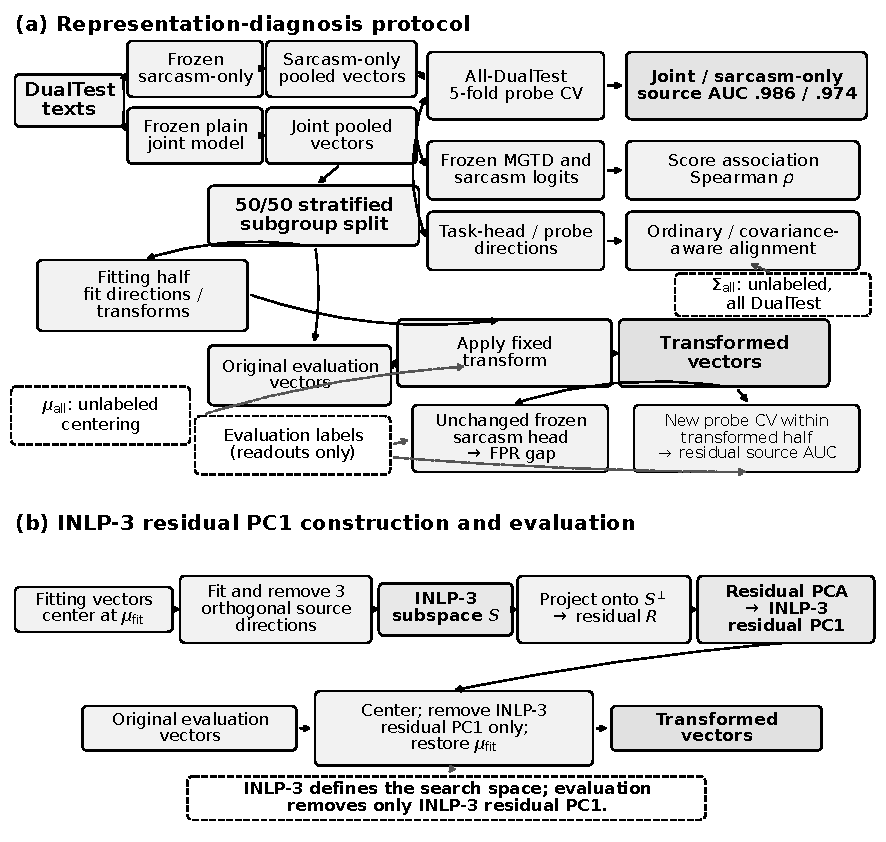
\includegraphics[width=\textwidth]{figures/fig_repr_protocol.pdf}
  \caption{Representation-diagnosis protocol. (a) Full-set probes are separate from split-sample interventions. Label-dependent directions and transformations use the fitting half, while covariance-aware alignment uses the full-set unlabeled covariance and specified Euclidean removals use the full-set unlabeled mean. Transformed evaluation vectors are read by the unchanged sarcasm head for source-group false-positive-rate gaps and by newly cross-validated source probes for residual linear source AUC. (b) INLP-3 defines the search space for the study-specific INLP-3 residual PC1; evaluation removes that PC1 alone from the original representations, not the INLP-3 subspace.}
  \label{fig:repr-protocol}
\end{figure*}

\phantomsection\label{app:e2}\paragraph{E.2 Probe, direction, and statistical protocols.} \Tabref{tab:repr-protocol} separates frozen representation sources, label-dependent estimation, unlabeled statistics, and evaluation readouts. Source probes use scikit-learn logistic regression with the \texttt{lbfgs} solver, $\ell_2$ penalty, $C=1.0$, no class weighting or feature scaling, and tolerance $10^{-4}$. AUC uses \texttt{cross\_val\_score} with five-fold stratified cross-validation, no shuffling, and ROC AUC scoring. Ordinary probes use at most 2{,}000 iterations; each INLP step uses at most 1{,}500.

\begin{table*}[!t]
  \centering
  \footnotesize
  \setlength{\tabcolsep}{2.5pt}
  \renewcommand{\arraystretch}{1.12}
  \begin{tabularx}{\textwidth}{@{}>{\raggedright\arraybackslash}p{1.85cm}>{\raggedright\arraybackslash}p{2.25cm}>{\raggedright\arraybackslash}X>{\raggedright\arraybackslash}X>{\raggedright\arraybackslash}X>{\raggedright\arraybackslash}p{2.0cm}@{}}
    \toprule
    \textbf{Component} & \textbf{Frozen source} & \textbf{Object derivation} & \textbf{Unlabeled statistics} & \textbf{Application /}\newline\textbf{evaluation} & \textbf{Readout or role} \\
    \midrule
    Full-set joint probe & Final plain joint vectors & Five-fold source-probe CV on all DualTest & None additionally specified & Held-out fold in full-set CV & Baseline source AUC 0.986 \\
    Full-set sarcasm-only probe & Matched sarcasm-only vectors & Same full-set CV protocol & None additionally specified & Held-out fold in full-set CV & Comparison AUC 0.974 \\
    Logit association & Final plain joint model & None & None & AI $\times$ non-sarcastic texts & Spearman correlation \\
    Task-head directions & Frozen joint task heads & Read $W_s[1]-W_s[0]$ and $W_a[0]-W_a[1]$ & $\Sigma_{\mathrm{all}}$ for alignment; $\mu_{\mathrm{all}}$ for Euclidean removal & Alignment; removal from evaluation vectors & Alignment; post-removal FPR gap and residual AUC \\
    Fitting-half probe direction & Joint fitting vectors & Logistic coefficient from fitting-half source labels & $\Sigma_{\mathrm{all}}$ for alignment; $\mu_{\mathrm{all}}$ for removal & Alignment; removal from evaluation vectors & Probe--head alignment; post-removal FPR gap and residual AUC \\
    INLP & Joint fitting vectors & Iterative source probes with orthogonalization & $\mu_{\mathrm{all}}$ & Remove $k\in\{1,2,4,8,16\}$ directions from evaluation vectors & Multi-direction Euclidean diagnostic; FPR gap and residual AUC \\
    LEACE & Joint fitting vectors & Fitting vectors and source labels & $\mu_{\mathrm{fit}},\Sigma_{\mathrm{fit}}$ & Fixed transform on evaluation vectors & Covariance-aware diagnostic; FPR gap and residual AUC \\
    INLP-3 residual PC1 & Joint fitting vectors & Labels fit INLP-3; residual PCA is unlabeled & $\mu_{\mathrm{fit}}$ and residual covariance & Remove PC1 only from original evaluation vectors & Residual-geometry diagnostic; FPR gap and residual AUC \\
    Post-intervention probe & Transformed evaluation vectors & Five-fold source-probe CV within each transformed set & None additionally specified & Held-out folds within transformed evaluation half & Residual source AUC \\
    \bottomrule
  \end{tabularx}
  \caption{Probe, direction-estimation, statistical, and post-intervention evaluation protocols. $\mu_{\mathrm{all}}$ and $\Sigma_{\mathrm{all}}$ use all unlabeled DualTest representations; $\mu_{\mathrm{fit}}$ and $\Sigma_{\mathrm{fit}}$ use the fitting half. Directional analyses omit the task-head bias, whereas predictions use the complete frozen head. Euclidean random controls use $\mu_{\mathrm{all}}$; covariance-whitened controls use fitting-half statistics. Object derivation states how each analysed object is obtained and whether source labels are used. Permuted-label and LEACE in-sample checks appear in E.5.}
  \label{tab:repr-protocol}
\end{table*}

Each task head is \texttt{Dropout} followed by \texttt{Linear(1024,2)}. For a binary linear head, the class-weight-row difference $d$ is its logit-contrast direction: for representation $z$, the positive-minus-negative logit has the form $d^{\top}z+\Delta b$, so moving $z$ along $d$ increases that contrast. The task-head directions are $d_{\mathrm{sarc}}=W_s[1]-W_s[0]$ for the sarcastic-minus-non-sarcastic logit and $d_{\mathrm{AI}}=W_a[0]-W_a[1]$ for the AI-minus-human logit (MGTD class 1 denotes human). Directional analyses omit bias; predictions use the complete head with dropout disabled in evaluation mode. For comparison, the fitting-half source probe supplies an independently estimated source direction: its $\ell_2$-normalized logistic-regression coefficient, oriented toward human authorship.

Ordinary cosine compares directions in Euclidean weight space. Covariance-aware alignment is $\cos(\Sigma_{\mathrm{all}}^{1/2}w_1,\Sigma_{\mathrm{all}}^{1/2}w_2)$, where $\Sigma_{\mathrm{all}}$ is the Ledoit--Wolf covariance \citep{ledoit2004covariance} of all pooled DualTest representations with eigenvalues clipped below $10^{-8}$. This use of all unlabeled representations makes the alignment transductive. Signed values are $-0.41197$ for the source-probe versus sarcasm directions and $+0.48713$ for the MGTD versus sarcasm directions; the main text reports absolute values because source-direction orientation changes the sign.

\paragraph{E.3 Intervention operators.} For representations $X$, selected mean $\mu$, and orthonormal direction matrix $U$, centered Euclidean removal is
\begin{equation}
  \mathcal{E}_{\mu}(X,U)=X-[(X-\mu)U]U^{\top},
  \label{eq:centered-erasure}
\end{equation}
which subtracts the selected component while retaining the mean. Task-head, source-probe, INLP, and Euclidean random removals use $\mu_{\mathrm{all}}$; LEACE, covariance-whitened controls, and INLP-3 residual PC1 use $\mu_{\mathrm{fit}}$.

INLP \citep{ravfogel2020inlp} repeatedly fits a source probe to the current fitting residuals, normalizes and Gram--Schmidt-orthogonalizes its coefficient, and deflates the representation. We evaluate $k\in\{1,2,4,8,16\}$ accumulated directions. Same-dimensional Euclidean random subspaces use QR-orthogonalized Gaussian matrices. These controls and permuted labels use \texttt{default\_rng(0)}.

LEACE \citep{belrose2023leace} is implemented directly. On the fitting half, let $\Sigma_{\mathrm{fit}}$ be the Ledoit--Wolf covariance with eigenvalues clipped below $10^{-8}$, and let $S_{xz}=X_c^{\top}Z_c/n$ for centered representations $X_c$ and centered one-hot source labels $Z_c$. We compute $M=\Sigma_{\mathrm{fit}}^{-1/2}S_{xz}$ and retain singular directions with $s>10^{-6}$, giving rank one. With whitened direction matrix $Q$, $P=\Sigma_{\mathrm{fit}}^{1/2}QQ^{\top}\Sigma_{\mathrm{fit}}^{-1/2}$ and erasure maps $X$ to $X-(X-\mu_{\mathrm{fit}})P^{\top}$. Ten covariance-whitened controls sample unit Gaussian $q$ and use $\Sigma_{\mathrm{fit}}^{1/2}qq^{\top}\Sigma_{\mathrm{fit}}^{-1/2}$.

For the exploratory, study-specific INLP-3 residual PC1, three fitting-half INLP directions define a low-dimensional source subspace $S$. The residual matrix is
\begin{equation}
  R=(X_{\mathrm{fit}}-\mu_{\mathrm{fit}})-[(X_{\mathrm{fit}}-\mu_{\mathrm{fit}})S]S^{\top}.
  \label{eq:srcorth-residual}
\end{equation}
The largest-eigenvalue vector of \texttt{np.cov}$(R^{\top})$ defines INLP-3 residual PC1. Evaluation applies Equation~\ref{eq:centered-erasure} to remove this single axis from the original evaluation vectors; the three INLP directions define the search space but are not themselves removed at evaluation time.

\phantomsection\label{app:repr-evidence}\paragraph{E.4 Diagnostic and intervention evidence.} This appendix records the full chain summarized in \Sref{sec:mechanism}. Q1 asks whether source is available in the representation, Q2 whether source-related quantities are associated with the sarcasm decision, and Q3 whether interventions change how the frozen sarcasm head allocates false positives across source groups. Source is highly linearly decodable: full-set AUC is 0.986 overall, 0.990 on sarcastic texts, and 0.985 on non-sarcastic texts; the matched sarcasm-only model yields 0.974. On AI $\times$ non-sarcastic texts, MGTD AI and sarcasm logits correlate at $\rho=0.519$, with length-tertile correlations of 0.44, 0.56, and 0.63. Task-head directions are nearly orthogonal under ordinary cosine ($\cos\approx-0.03$), whereas covariance-aware absolute alignment is 0.49 for the MGTD-head direction and 0.41 for the fitting-half source-probe direction. These results associate source-related scores and data-weighted directions with the affected decisions.

For interventions, $\text{gap}$ is AI minus human FPR on non-sarcastic evaluation texts; source AUC is obtained from a new probe cross-validated within each transformed evaluation set. The untouched baseline is 84.788\% AI FPR and 32.774\% human FPR (gap 52.014 pp), with source AUC 0.98197.

\begin{table*}[!t]
  \centering
  \footnotesize
  \setlength{\tabcolsep}{6pt}
  \begin{tabularx}{0.78\textwidth}{@{}>{\raggedright\arraybackslash}Xcccc@{}}
    \toprule
    \textbf{Erasure scheme} & \textbf{AI$\times$n FPR} & \textbf{H$\times$n FPR} & \textbf{Gap} & \textbf{AUC} \\
    \midrule
    None (baseline) & 84.8 & 32.8 & 52.0 & 0.982 \\
    MGTD-head direction & 86.2 & 30.2 & 56.0 & 0.982 \\
    Source-probe direction & 84.8 & 32.9 & 51.9 & 0.981 \\
    Euclidean random direction & 85.2 & 32.6 & 52.5 & 0.982 \\
    INLP ($k = 16$) & 89.8 & 17.7 & 72.1 & 0.974 \\
    \textbf{LEACE (linear)} & 68.7 & 49.5 & 19.1 & \textbf{0.589} \\
    Whitened random $\times$10 (mean) & 84.9 & 32.7 & 52.2 & 0.982 \\
    \textbf{INLP-3 residual PC1} & \textbf{66.7} & 54.1 & 12.6 & \textbf{0.982} \\
    \bottomrule
  \end{tabularx}
  \caption{Intervention summary. H$\times$n = human $\times$ non-sarcastic; AI$\times$n = AI $\times$ non-sarcastic; FPR in \%; gaps use unrounded rates. Whitened-control values average ten directions, whose gaps range from 51.4 to 52.7 pp. AUC is the newly cross-validated post-intervention source-probe AUC.}
  \label{tab:intervention}
\end{table*}

\Tabref{tab:intervention} summarizes the interventions. The MGTD-head, source-probe, Euclidean-random, and INLP interventions do not narrow the gap; INLP at $k=16$ widens it to 72.1 pp. Their residual source AUC also remains above 0.97, so these operators do not remove source in the first place, and their effect on the gap is uninformative about whether source matters. LEACE lowers measured source AUC to 0.589 and the gap to 19.1 pp; no whitened random direction produces a comparable change. These controls nevertheless perturb representations far less than LEACE does---mean relative change 0.02 against 0.53---so they establish only that an arbitrary whitened direction is insufficient and do not separate erasing source from perturbing the representation strongly. The INLP-3 residual PC1 condition supplies that separation: its mean relative change is 0.57, comparable to LEACE, yet it leaves source AUC at 0.982. The unweighted mean FPR of the two source groups is nearly unchanged (58.8 $\to$ 59.1) because the human non-sarcastic rate rises from 32.8 to 49.5, showing error reallocation rather than lower average error.

Removing INLP-3 residual PC1 changes AI FPR to 66.7 and the gap to 12.6 pp while source AUC remains 0.982. The new probe can recover source from the remaining representation even though removing this axis reallocates errors across the two source groups. Together with the LEACE result, this shows that the FPR gap is not determined by residual linear source AUC alone: both covariance-aware source structure and a residual high-variance axis can affect how the fixed sarcasm head distributes errors between source groups.

\paragraph{E.5 Implementation checks.} Manually computed logits match model outputs with maximum error $1.4\times10^{-6}$, and projection residuals are about $10^{-6}$. LEACE leaves a fitting-half class-mean residual of $7\times10^{-6}$ and fitting-half probe AUC 0.514; these are implementation checks, not held-out results. A permuted-label full-set probe gives AUC 0.512. Thus, the reported AUCs refer to distinct settings: 0.986 is full-set five-fold baseline decodability, 0.982 is the untouched intervention-half baseline, 0.514 is the LEACE in-sample check, and 0.589 is held-out post-LEACE decodability.
